%!TEX root = main.tex

\section{Definitions and key notation}\label{sec:dfin}

We use three notations for working with probability theory. The ``elementary'' notation makes use of regular symbolic conventions (functions, products, sums, integrals, unions etc.) along with the expectation operator $\mathbb{E}$. This is the most flexible notation which comes at the cost of being verbose and difficult to read. Secondly, we use a semi-formal string diagram notation extending the formal diagram notation for symmetric monoidal categories \cite{selinger_survey_2010}. Objects in this diagram refer to stochastic maps, and by interpreting diagrams as symbols we can, in theory, be just as flexible as the purely symbolic approach. However, we avoid complex mixtures of symbols and diagrams elements, and fall back to symbolic representations if it is called for. Finally, we use a matrix-vector product convention that isn't particularly expressive but can compactly express some common operations.

\subsection{Standard Symbols}

\begin{center}
\begin{tabular}{ |c|c|c| } 
 \hline
 Symbol & Meaning \\ 
 $[n]$& The natural numbers $\{1,...,n\}$ \\ 
 $f:a\mapsto b$ & Function definition, equivalent to $f(a):=b$\\
 Dots appearing in function arguments: $f(\cdot,\cdot,z)$ & The ``curried'' function $(x, y )\mapsto f(x,y,z)$\\
 Capital letters: $A,B, X$ & sets \\ 
 Script letters: $\mathcal{A},\mathcal{B},\mathcal{X}$ & $\sigma$-algebras on the sets $A, B, X$ respectively\\
 Script $\mathcal{G}$ & A directed acyclic graph made up of nodes $V$ and edges $E$\\
 Greek letters $\mu, \xi, \gamma$ & Probability measures\\
 $\delta_x$ & The Dirac delta measure: $\delta_x(A) = 1$ if $x\in A$ and $0$ otherwise\\
 Capital delta: $\Delta(\mathcal{E})$ & The set of all probability measures on $\mathcal{E}$\\
 Bold capitals: $\mathbf{A}$ & Markov kernel $\mathbf{A}:X\times\mathcal{Y}\to [0,1]$ (stochastic maps)\\
 Subscripted bold capitals: $\mathbf{A}_x$ & The probability measure given by the curried Markov kernel $\mathbf{A}(x,\cdot)$\\
 $A\to\Delta(\mathcal{B})$ & Markov kernel signature, treated as equivalent to $A\times \mathcal{B}\to [0,1]$\\
 $\mathbf{A}:x\mapsto \nu$ & Markov kernel definition, equivalent to $\mathbf{A}(x,B) = \nu(B)$ for all $B$\\
 Sans serif capitals: $\RV{A},\RV{X}$ & Measurable functions; we will also call them random variables\\
 $\mathbf{F}_{\RV{X}}$ & The Markov kernel associated with the function $\RV{X}$: $\mathbf{F}_{\RV{X}} \equiv a\mapsto \delta_{\RV{X}(a)}$\\
 $\mathbf{N}_{\RV{A}|\RV{B}}$ & The conditional probability (disintegration) of $\RV{A}$ given $\RV{B}$ under $\nu$\\
 $\nu \mathbf{F}_{\RV{X}}$ & The marginal distribution of $\RV{X}$ under $\nu$\\
 \hline
\end{tabular}
\end{center}

\subsection{Probability Theory}

Given a set $A$, a $\sigma$-algebra $\mathcal{A}$ is a collection of subsets of $A$ where
\begin{itemize}
	\item $A\in \mathcal{A}$ and $\emptyset\in \mathcal{A}$
	\item $B\in \mathcal{A}\implies B^C\in\mathcal{A}$
	\item $\mathcal{A}$ is closed under countable unions: For any countable collection $\{B_i|i\in Z\subset \mathbb{N}\}$ of elements of $\mathcal{A}$, $\cup_{i\in Z}B_i\in \mathcal{A}$ 
\end{itemize}

A measurable space $(A,\mathcal{A})$ is a set $A$ along with a $\sigma$-algebra $\mathcal{A}$. Sometimes the sigma algebra will be left implicit, in which case $A$ will just be introduced as a measurable space.

\paragraph{Common $\sigma$ algebras}

For any $A$, $\{\emptyset,A\}$ is a $\sigma$-algebra. In particular, it is the only sigma algebra for any one element set $\{*\}$.

For countable $A$, the power set $\mathscr{P}(A)$ is known as the discrete $\sigma$-algebra.

Given $A$ and a collection of subsets of $B\subset\mathscr{P}(A)$, $\sigma(B)$ is the smallest $\sigma$-algebra containing all the elements of $B$. 

Let $T$ be all the open subsets of $\mathbb{R}$. Then $\mathcal{B}(\mathbb{R}):=\sigma(T)$ is the \emph{Borel $\sigma$-algebra} on the reals. This definition extends to an arbitrary topological space $A$ with topology $T$.

A \emph{standard measurable set} is a measurable set $A$ that is isomorphic either to a discrete measurable space $A$ or $(\mathbb{R}, \mathcal{B}(\mathbb{R}))$. For any $A$ that is a complete separable metric space, $(A,\mathcal{B}(A))$ is standard measurable. 

Given a measurable space $(E,\mathcal{E})$, a map $\mu:\mathcal{E}\to [0,1]$ is a \emph{probability measure} if
\begin{itemize}
	\item $\mu(E)=1$, $\mu(\emptyset)=0$
	\item Given countable collection $\{A_i\}\subset\mathscr{E}$, $\mu(\cup_{i} A_i) = \sum_i \mu(A_i)$
\end{itemize}

Write by $\Delta(\mathcal{E})$ the set of all probability measures on $\mathcal{E}$.

Given a second measurable space $(F,\mathcal{F})$, a \emph{stochastic map} or \emph{Markov kernel} is a map $\mathbf{M}:E\times\mathcal{F}\to [0,1]$ such that
\begin{itemize}
	\item The map $\mathbf{M}(\cdot;A):x\mapsto \mathbf{M}(x;A)$ is $\mathcal{E}$-measurable for all $A\in \mathcal{F}$
	\item The map $\mathbf{M}_x:A\mapsto \mathbf{M}(x;A)$ is a probability measure on $F$ for all $x\in E$
\end{itemize}

Extending the subscript notation above, for $\mathbf{C}:X\times Y\to \Delta(\mathcal{Z})$  and $x\in X$ we will write $\mathbf{C}_x$ for the ``curried'' map $y\mapsto \mathbf{C}_{x,y}$.

The map $x\mapsto \mathbf{M}_x$ is of type $E\to \Delta(\mathcal{F})$. We will abuse notation somewhat to write $\mathbf{M}:E\to \Delta(\mathcal{F})$, which captures the intuition that a Markov kernel maps from elements of $E$ to probability measures on $\mathcal{F}$. Note that we ``reverse'' this idea and consider Markov kernels to map from elements of $\mathcal{F}$ to measurable functions $E\to[0,1]$, an interpretation found in \citet{clerc_pointless_2017}, but (at this stage) we don't make use of this interpretation here.

Given an indiscrete measurable space $(\{*\},\{\{*\},\emptyset\})$, we identify Markov kernels $\mathbf{N}:\{*\}\to \Delta(\mathcal{E})$ with the probability measure $\mathbf{N}_*$. In addition, there is a unique Markov kernel $\stopper{0.2}:E\to \Delta(\{\{*\},\emptyset\})$ given by $x\mapsto \delta_*$ for all $x\in E$ which we will call the ``discard'' map.


\subsection{Product Notation}

We can use a notation similar to the standard notation for matrix-vector products to represent operations with Markov kernels. Probability measures $\mu\in \Delta(\mathcal{X})$ can be read as row vectors, Markov kernels as matrices and measurable functions $\RV{T}:Y\to T$ as column vectors. Defining $\mathbf{M}:X\to \Delta(\mathcal{Y})$ and $\mathbf{N}:Y\to \Delta(\mathcal{Z})$, the measure-kernel product $\mu \mathbf{A} (G) := \int \mathbf{A}_x (G) d\mu(x)$ yields a probability measure $\mu\mathbf{A}$ on $\mathcal{Z}$, the kernel-kernel product $\mathbf{M}\mathbf{N}(x;H)=\int_Y \mathbf{B}(y;H)d\mathbf{A}_x$ yields a kernel $\mathbf{M}\mathbf{N}:X\to \Delta(\mathcal{Z})$ and the kernel-function product $\mathbf{A}\RV{T}(x):=\int_Y \RV{T}(y) d\mathbf{A}_x$ yields a measurable function $X\to T$. Kernel products are associative \citep{cinlar_probability_2011}.

The tensor product $(\mathbf{M}\otimes \mathbf{N})(x,y;G,H) := \mathbf{M}(x;G)\mathbf{N}(y;H)$ yields a kernel $(\mathbf{M}\otimes \mathbf{N}):X\times Y\to \Delta(\mathcal{Y}\otimes\mathcal{Z})$.

\subsection{String Diagrams}

Some constructions are unwieldly in product notation; for example, given $\mu\in \Delta(\mathcal{E})$ and $\mathbf{M}:E\to (\mathcal{F})$, it is not straightforward to construct a measure $\nu\in\Delta(\mathcal{E}\otimes\mathcal{F})$ that captures the ``joint distribution'' given by $A\times B\mapsto \int_A \mathbf{M}(x;B)d\mu$. 

Such constructions can, however, be straightforwardly captured with string diagrams, a notation developed for category theoretic probability. \citet{cho_disintegration_2019} also provides an extensive introduction to the notation discussed here.

Some key ideas of string diagrams:
\begin{itemize}
	\item Basic string diagrams can always be interpreted as a mixture of kernel-kernel products and tensor products of Markov kernels
	\begin{itemize}
	\item Extended string diagrams can be interepreted as a mixture of kernel-kernel products, kernel-function products, tensor products of kernels and functions and scalar products 
	\end{itemize}
	\item String diagrams are the subject of a coherence theorem: taking a string diagram and applying a planar deformation yields a string diagram that represents the same kernel \citep{selinger_survey_2010}. This also holds for a number of additional transformations detailed below
\end{itemize}

A kernel $\mathbf{M}:X\to \Delta(\mathcal{Y})$ is written as a box with input and output wires, probability measures $\mu\in \Delta(\mathcal{X})$ are written as triangles ``closed on the left'' and measurable functions (which are only elements of the ``extended'' notation) $\RV{T}:Y\to T$ as triangles ``closed on the right''. We additionally name every wire represented in a string diagram, which we call (following \cite{cho_disintegration_2019}) \emph{meta-variables} and use the same sans-serif font as for random variabels ($\RV{X},\RV{Y}$ etc.) to emphasise their connection. See Paragraph \ref{par:random_variables} for a more detailed explanation of meta variables.

For $\mathbf{M}:X\to \Delta(\mathcal{Y})$, $\mu\in \Delta(\mathcal{X})$ and $f:X\to W$:

\begin{align}
\begin{tikzpicture}
\path (0,0) node (A) {$\RV{X}$}
++(0.75,0) node[kernel] (B) {$\mathbf{M}$}
++(0.75,0) node (C) {$\RV{Y}$};
\draw (A) -- (B) -- (C);
\end{tikzpicture}\qquad
\begin{tikzpicture}
\path (0,0) node[dist] (B) {$\mu$}
++(0.75,0) node (C) {$\RV{X}$};
\draw (B) -- (C);
\end{tikzpicture}\qquad
\begin{tikzpicture}
\path (0,0) node (A) {$\RV{X}$}
++(0.75,0) node[expectation] (B) {$f$};
\draw (A) -- (B);
\end{tikzpicture}
\end{align}

\paragraph{Basic and extended notation}

We canonically regard a probability measure $\mu\in \Delta(\mathcal{E})$ to be a Markov kernel $\mu:\{*\}\to \Delta(\mathcal{E})$. This allows for the definition of ``basic'' string diagrams for which Markov kernels are the only building blocks. Such a definition isn't possible for measurable functions. Suppose by analogy with the example probability measures and try to identify a measurable function $f:E\to \mathbb{R}$ with a Markov kernel $f':E\times\{*\}\to \mathbb{R}$. For $x\in E$ we cannot generally have both $f'(x,*)=1$ and $f'(x,*)=f(x)$, and so this attempt fails. This lack of normalisation is the reason we require an ``extended'' string diagram notation if we wish to incorporate functions and expectations which allows for the representation of scalars.


\paragraph{Elementary operations}

We can compose Markov kernels with appropriate spaces - the equivalent operation of the ``matrix products'' of product notation. Given $\mathbf{M}:X\to\Delta(\mathcal{Y})$ and $\mathbf{N}:Y\to \Delta(\mathcal{Z})$, we have 

\begin{align}
\mathbf{M}\mathbf{N} := \begin{tikzpicture}
 \path (0,0) node (E) {$\RV{X}$}
 ++ (1,0) node[kernel] (M) {$\mathbf{M}$}
 ++ (1,0) node[kernel] (N) {$\mathbf{N}$}
 ++(1,0) node (G) {$\RV{Z}$};
 \draw (E) -- (M) -- (N) -- (G);
\end{tikzpicture}\label{eq:sd_composition}
\end{align}

Probability measures are distinguished in that that they only admit ``right composition'' while functions only admit ``left composition''. For $\mu\in \Delta(\mathcal{E})$, $h:F\to X$:

\begin{align}
\mu\mathbf{M} &:= \begin{tikzpicture}
 \path (0,0) node[dist] (M) {$\mu$}
 ++ (1,0) node[kernel] (N) {$\mathbf{M}$}
 ++(1,0) node (G) {$\RV{Z}$};
 \draw (M) -- (N) -- (G);
\end{tikzpicture}\\
\mathbf{M}f&:= \begin{tikzpicture}
 \path (0,0) node (E) {$\RV{X}$}
 ++ (1,0) node[kernel] (M) {$\mathbf{M}$}
 ++ (1,0) node[expectation] (N) {$f$};
 \draw (E) -- (M) -- (N);
 \end{tikzpicture}
\end{align}


We can also combine Markov kernels using tensor products, which we represent with vertical juxtaposition. For $\mathbf{O}:Z\to \Delta(\mathcal{W})$:


\begin{align}
\mathbf{M}\otimes\mathbf{N}&:= \begin{tikzpicture}
\path (0,0) node (E) {$\RV{X}$}
++(1,0) node[kernel] (M) {$\mathbf{M}$}
++(1,0) node (F) {$\RV{Y}$}
(0,-0.5) node (F1) {$\RV{Z}$}
++(1,0) node[kernel] (N) {$\mathbf{O}$}
+(1,0) node (G) {$\RV{W}$};
\draw (E) -- (M) -- (F);
\draw (F1) -- (N) -- (G);
\end{tikzpicture}
\end{align}

Product spaces can be represented either by two parallel wires or a single wire:
\begin{align}
X\times Y \cong \mathrm{Id}_X\otimes \mathrm{Id}_Y &:= 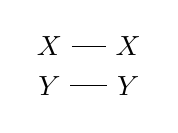
\begin{tikzpicture}
\path (0,0) node (E) {$\RV{X}$}
++(1,0) node (F) {$\RV{X}$}
(0,-0.5) node (F1) {$\RV{Y}$}
+(1,0) node (G) {$\RV{Y}$};
\draw (E) -- (F);
\draw (F1) -- (G);
\end{tikzpicture}\\
&= 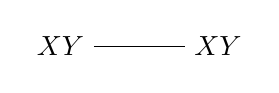
\begin{tikzpicture}
\path (0,0) node (X) {$\RV{X}\utimes \RV{Y}$}
++(2,0) node (Y) {$\RV{X}\utimes \RV{Y}$};
\draw (X) -- (Y);
\end{tikzpicture}
\end{align}

The notation $\RV{X}\utimes \RV{Y}$ will be explained in paragraph \ref{pgph:disint} - $\RV{X}\utimes\RV{Y}$ is a meta variable taking values in in the product space $X\times Y$.

Because a product space can be represented by parallel wires, a kernel $\mathbf{L}:X\to \Delta(\mathcal{Y}\otimes\mathcal{Z})$ can be written using either two parallel output wires or a single output wire:

\begin{align}
&\begin{tikzpicture}
\path (0,0) node (E) {$\RV{X}$}
++ (1,0) node[kernel] (L) {$\mathbf{L}$}
++ (1,0.15) node (F) {$\RV{Y}$}
+(0,-0.3) node (G) {$\RV{Z}$};
\draw (E) -- (L);
\draw ($(L.east) + (0,0.15)$) -- (F);
\draw ($(L.east)+ (0,-0.15)$) -- (G);
\end{tikzpicture}\\
&\equiv\\
&\begin{tikzpicture}
\path (0,0) node (E) {$\RV{X}$}
++ (1,0) node[kernel] (L) {$\mathbf{L}$}
++ (1.5,0) node (F) {$\RV{Y}\utimes \RV{Z}$};
\draw (E) -- (L) -- (F);
\end{tikzpicture}
\end{align}


\paragraph{Markov kernels with special notation}

A number of Markov kernels are given special notation distinct from the generic ``box'' representation above. These special representations facilitate intuitive graphical interpretations.

The identity kernel $\textbf{Id}:X\to \Delta(X)$ maps a point $x$ to the measure $\delta_x$ that places all mass on the same point:

\begin{align}
\textbf{Id}_x : x\mapsto \delta_x \equiv \begin{tikzpicture}\path (0,0) node (X) {$\RV{X}$} + (1,0) node (X1) {$\RV{X}$}; \draw (X)--(X1); \end{tikzpicture}
\end{align}

The identity map preserves the name of a wire.

The copy map $\splitter{0.1}:X\to \Delta(\mathcal{X}\times \mathcal{X})$ maps a point $x$ to two identical copies of x:
\begin{align}
 \splitter{0.1}: x\mapsto \delta_{(x,x)} \equiv 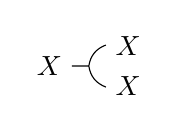
\begin{tikzpicture}
 \path (0,0) node (X) {$X$} ++ (0.5,0) coordinate (copy0) ++ (0.5,0.25) node (X1) {$\RV{X}$} ++(0,-0.5) node (X2) {$\RV{X}$};\draw (X)--(copy0) to [bend left] (X1) (copy0) to [bend right] (X2);
 \end{tikzpicture}
 \end{align} 

Copy maps \emph{copy} the name of a wire. 

The swap map $\sigma:X\times Y\to \Delta(\mathcal{Y}\otimes\mathcal{X})$ swaps its inputs:

\begin{align}
\sigma := (x,y)\to \delta_{(y,x)} \equiv 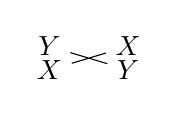
\begin{tikzpicture}
\path (0,0) node (X) {$\RV{X}$}
+(1,0.3) node (X1) {$\RV{X}$}
(0,0.3) node (Y) {$\RV{Y}$}
+(1,-0.3) node (Y1) {$\RV{Y}$};
\draw (X)--(X1) (Y) -- (Y1);
\end{tikzpicture}
\end{align}

The swap map preserves the names of visually connected wires.

Apart from identity, copy and swap maps, we assign different names to the input and output wires of Markov kernels.

The discard map $\stopper{0.2}:X\to \Delta(\{*\})$ maps every input to $\delta_{*}$ which is effectively mapping every input to 1
\begin{align}
\stopper{0.2}: x\mapsto \delta_{*} \equiv \begin{tikzpicture}
 \draw[-{Rays [n=8]}] (0,0) node (X) {$\RV{X}$} (X) -- (1,0);
\end{tikzpicture}
\end{align}

Before introducing key rules of manipulation permitted by string diagrams, we will illustrate the correspondence between the three notations with a few simple examples. Given $\mu\in\Delta(X),\mathbf{A}:X\to \Delta(Y)$ and $A\in \mathcal{X}$, $B\in\mathcal{Y}$, the following correspondences hold, where we express the same object in elementary notation, product notation and string notation respectively:

\begin{align}
\nu:=A\times B\mapsto \int_A A(x;B)d\mu(x) \equiv \mu \splitter{0.1}(\textbf{Id}_X\otimes \mathbf{A}) \equiv  \begin{tikzpicture}
\path (0,0) node[dist] (mu) {$\mu$}
++ (1,0) coordinate (copy0)
+ (1.2,0.5) node (X) {$\RV{X}$}
++ (0.5,-0.5) node[kernel] (A) {$\mathbf{A}$}
++(0.7,0) node (Y) {$\RV{Y}$};
\draw (mu)--(copy0);
\draw (copy0) to [bend left] (X);
\draw (copy0) to [bend right] (A) (A) -- (Y);
\end{tikzpicture}\label{eq:joint_measure}
\end{align}

Where the resulting object is a probability measure $\nu\in \Delta(\mathcal{X}\otimes\mathcal{Y})$. Note that the elementary notation requires a function definition here, while the product and string notations can represent the measure without explicitly addressing its action on various inputs and outputs. \citet{cho_disintegration_2019} calls this construction ``integrating $\mathbf{A}$ with respect to $\mu$''.

Define the marginal $\nu_Y\in \Delta(\mathcal{Y}):B\mapsto \nu(X\times B)$ for $B\in \mathcal{Y}$ and similarly for $\nu_X$. We can then express the result of marginalising \ref{eq:joint_measure} over $X$ in our three separate notations as follows:
\begin{align}
  \nu_Y (B) &= \nu(X\times B) = \int_X A(x;B) d\mu(x)\label{eq:marginalisation_elem}\\
  \nu_Y &= \mu \mathbf{A} = \mu \splitter{0.1}(\textbf{Id}_X\otimes \mathbf{A})(\stopper{0.2}\otimes \textbf{Id}_Y)\label{eq:marginalisation_prod}\\
  \nu_Y &= \begin{tikzpicture}
\path (0,0) node[dist] (mu) {$\mu$} ++ (1,0) node[kernel] (A) {$\mathbf{A}$} ++ (0.7,0) node (Y) {$\RV{Y}$}; \draw (mu) -- (A) -- (Y);
\end{tikzpicture} = \begin{tikzpicture}
\path (0,0) node[dist] (mu) {$\mu$}
++ (1,0) coordinate (copy0)
+ (1.2,0.5) node (X) {}
++ (0.5,-0.5) node[kernel] (A) {$\mathbf{A}$}
++(0.7,0) node (Y) {$\RV{Y}$};
\draw (mu)--(copy0);
\draw[-{Rays [n=8]}] (copy0) to [bend left] (X);
\draw (copy0) to [bend right] (A) (A) -- (Y);
\end{tikzpicture}\label{eq:marginalisation_graph}
\end{align}

The elementary notation \ref{eq:marginalisation_elem} makes the relationship between $\nu_Y$ and $\nu$ explicit and, again, requires the action on each event to be defined. The product notation \ref{eq:marginalisation_prod} is, in my view, the least transparent but also the most compact in the form $\mu \mathbf{A}$, and does not demand the explicit definition of how $\nu_Y$ treats every event. The graphical notation is the least compact in terms of space taken up on the page, but unlike the product notation it shows a clear relationship to the graphical construction in\ref{eq:joint_measure}, and displays a clear graphical logic whereby marginalisation corresponds to ``cutting off branches''. Like product notation, it also allows for the definition of derived measures such as $\nu_Y$ without explicit definition of the handling of all events. It also features a much smaller collection of symbols than does elementary notation.

String diagrams often achieve a good balance between interpretational transparency, expressive power and symbol economy. Downsides of string diagrams are that they can be time consuming to typeset, and formal reasoning with them takes some practice.


\subsubsection{Meta Variables}\label{par:random_variables}


If all our reasoning were done using diagrams wire identities would be clear from those diagrams. However, because we reason using a combination of diagrams, product notation, elementary notation and English words, it is necessary to be able to refer to particular wires in a diagram. We call wire labels \emph{meta variables}, which are closely connected to the more standard \emph{random variables}. Given a diagram representing a probability measure (rather than a general Markov kernel) that defines a number of meta variables, we can take the marginal distribution of a given meta variable or find the conditional distribution of one set of meta variables given another. In addition, we can perform analogous operations to marginalisation and finding the conditional distribution of meta variables for general Markov kernels.

\paragraph{Meta variables and probability measures}


Given a probability measure $\mu\in \Delta(\mathcal{X}\otimes\mathcal{Y})$, a \emph{meta variable} is a label attached to an output wire of the diagram in some valid representation. By convention, we name meta variables with sans-serif letters matching the name of the underlying space, though this is only a convention. For example, the following two diagrams define meta variables $\RV{X}$, $\RV{Y}$ and $\RV{W}$:
\begin{align}
&\begin{tikzpicture}
\path (0,0) node[dist] (M) {$\mu$}
++ (0.7,0.15) node (X) {$\RV{X}$}
++ (0,-0.3) node (Y) {$\RV{Y}$};
\draw ($(M.east)+(0,0.15)$) -- (X);
\draw ($(M.east)+(0,-0.15)$) -- (Y);
\end{tikzpicture} &
\begin{tikzpicture}
\path (0,0) node[dist] (M) {$\mu$}
++ (0.7,0) node (W) {$\RV{W}$};
\draw (M) -- (W);
\end{tikzpicture}
\end{align}

We insist that meta variables obey a number of consistency properties which ensure that wires that are intuitively the same between diagrams receive the same label.

We take a slightly nonstandard view of random variables. Random variables are typically defined to be measurable functions on a probability space $\langle \Omega, \mathcal{F}, \mu\rangle$ \citep{cinlar_probability_2011}. With this definition, a random variable $\RV{X}:\Omega\to E$ has a canonical probability measure given by the pushforward of $\mu$: for all $A\in\mathscr{E}$ $\RV{X}_\# \mu(A) = \mu(\RV{X}^{-1}(A))$.

We take a random variable to be a measurable function on a \emph{kernel space} $\langle F, G, \mathcal{F}\otimes\mathcal{G},\mathbf{M}\rangle$ where $\mathbf{M}:G\to \Delta(\mathcal{F})$ is a Markov kernel. A random variable $\RV{X}:F\to X$ has a probability distribution only relative to some argument measure $\nu\in\Delta(\mathcal{G})$. Because of this, we cannot in general unambiguously talk about ``the'' distribution of a given random variable; in general we have only conditional probabilities (which we define in Paragraph \ref{pgph:disint}). This approach mirrors to some extent the approach suggested by \citet{hajek_what_2003}, which also takes conditional probability to be fundamental.

This choice is largely pragmatic - it is helpful to make statements about the properties of random variables on a kernel space without quantifying over prior distributions. However, there is a connection between this choice and the philosophical field of decision theory. In particular, we use random variables to model both stochastic quantities and quantities that depend on the decision maker's choices. We treat the uncertainty associated with choosing and that associated with stochasticity as different -- we do \emph{not} suppose that uncertainty over which choice will be made should itself be modeled using probability. \emph{Evidential decision theory}, as defended by \citet{jeffrey_logic_1981}, proposes that is is proper to consider choices to be random variables, though it  doing so rigorously may necessitate a theory that allows for the assignment of probabilities to the outcomes of mathematical deliberations such as the theory of \emph{logical induction} introduced in \citet{garrabrant_logical_2017}. Understanding the relationship between choices and stochastic processes is a deep, interesting and difficut question, and one we sidestep by presuming that we can address nearly all common decision problems while disregarding modelling whatever process gives rise to choices. The resulting decision theory is structurally similar to \emph{causal decision theory} \citep{lewis_causal_1981}.

This definition of random variables permits the convention of identifying every output wire of a string diagram with a random variable. 

\begin{definition}[Function induced kernel]
Given a measurable function $\RV{X}:F\to X$, define the function induced kernel $\mathbf{F}_{\RV{X}}:F\to \Delta(\mathcal{X})$ to the the Markov kernel $a\mapsto \delta_{\RV{X}(a)}$ for all $a\in X$.
\end{definition}

\begin{lemma}[Pushforward measures and functional kernels]\label{lem:pushf_funk}
Given a kernel space $\langle F,\mathcal{F},\mathbf{M}, G\rangle$ and a random variable $\RV{X}:F\to X$, for any prior $\mu\in \Delta(\mathcal{G})$ the pushforward $\RV{X}_\# \mu \mathbf{A} = \mu\mathbf{A} \mathbf{F}_{\RV{X}}$.
\end{lemma}

\begin{proof}
For all $B\in \mathcal{F}$:
\begin{align}
  (\RV{X})_\# \mu \mathbf{A} (B) &= \mu \mathbf{A} (\RV{X}^{-1}(B))\\
  								   &= \int_{F} \delta_{\RV{X}(a)} (B) d\mu\mathbf{A} (a)\\
  								   &= \mu\mathbf{A}\mathbf{F}_{\RV{X}}(B)
\end{align}
\end{proof}

\begin{example}[Wire names to random variables]
Suppose we have a Markov kernel $\mathbf{A}:X\to \Delta(\mathcal{Y}\otimes\mathcal{Y})$:
\begin{align}
\begin{tikzpicture}
\path (0,0) node (A) {$X$}
++(0.75,0) node[kernel] (B) {$\mathbf{A}$}
++(0.75,0.15) node (C) {$\RV{Y}_1$}
+(0,-0.3) node (D) {$\RV{Y}_2$};
\draw (A) -- (B) ($(B.east) + (0,0.15)$) -- (C) ($(B.east)+(0,-0.15)$) -- (D);
\end{tikzpicture}
\end{align}

Define $\RV{Y}'_1:Y\times Y\to Y$ by the projection map $\RV{Y}'_1:(y_1,y_2)\mapsto y_1$ and $\RV{Y}'_2:Y\times Y\to Y$ by the projection $\RV{Y}'_2:(y_1,y_2)\mapsto y_2$. Given any prior $\mu\in \Delta(\mathcal{X})$, let $(\RV{Y}'_1)_\# \mu \mathbf{A}$ be the pushforward of $\RV{Y}'_1$ by $\mu\mathbf{A}$. Then $\mathbf{F}_{\RV{Y}'_1}:Y\times Y\to Y$ will be given by $a\mapsto \delta_{\RV{Y}'_1(a)}$.

Define $\Pi_{\RV{Y}_1}:Y\times Y\to \Delta(\mathcal{Y})$ by $\Pi_{\RV{Y}_1}=\mathrm{Id}_Y\otimes \stopper{0.2}$. $\Pi_{\RV{Y}_1}$ is the Markov kernel that marginalises over the second argument; i.e. it marginalises over the wire named $\RV{Y}_2$. Graphically:

\begin{align}
\mathbf{A}\Pi_{\RV{Y}_1} = 
\begin{tikzpicture}
\path (0,0) node (A) {$X$}
++(0.75,0) node[kernel] (B) {$\mathbf{A}$}
++(1,0.15) node (C) {$\RV{Y}_1$}
+(-0.25,-0.3) node (D) {};
\draw (A) -- (B) ($(B.east) + (0,0.15)$) -- (C);
\draw[-{Rays[ n=8]}] ($(B.east)+(0,-0.15)$) -- (D);
\end{tikzpicture}
\end{align}

Note that for all $(y_1,y_2)\in Y\times Y$, $(\Pi_1)_{y_1,y_2} = \delta_{y_1} = \delta_{\RV{Y}'_1(y_1,y_2)}$. That is, $\Pi_{\RV{Y}_1}=F_{\RV{Y}'_1}$ and so $(\RV{Y}'_1)_\# \mu\mathbf{A} = \mu\mathbf{A}\Pi_{\RV{Y}_1}$. 

Furthermore, define the joint distribution of $\RV{Y}'_1$ and $\RV{Y}'_2$ by $(\RV{Y}'_{1}\utimes\RV{Y}'_{2})_\# \mu\mathbf{A}(B\times C) = \mu\mathbf{A}(\RV{Y}_1^{\prime-1}(B)\cap \RV{Y}_2^{\prime-1}(C))$ for all $B,C\in \mathcal{Y}$. Then, defining $\Pi_{\RV{Y}_1\otimes\RV{Y}_2} = \mathrm{Id}_Y\otimes \mathrm{Id}_Y = \mathrm{Id}_{Y\times Y}$:

\begin{align}
 (\RV{Y}'_1\utimes\RV{Y}'_2)_\# \mu\mathbf{A}(B\times C) &= \mu\mathbf{A}(\RV{Y}_1^{\prime-1}(B)\cap \RV{Y}_2^{\prime-1}(C))\\
 													   &= \int_{Y\times Y} \delta_{\RV{Y}'_1(y_1,y_2)}(B) \delta_{\RV{Y}'_2(y_1,y_2)}(C) d\mu\mathbf{A}(y_1,y_2)\\
 													   &= \int_{B\times C} d\mu\mathbf{A}(y_1,y_2)\\
 													   &= \mu\mathbf{A}(B\times C)\\
 													   &= \mu\mathbf{A}\Pi_{\RV{Y}_1\otimes\RV{Y}_2} (B\times C) \label{eq:identity}
\end{align}

That is, for any prior $\mu$, the joint distribution of $\RV{Y}'_1$ and $\RV{Y}'_2$ under $\mu\mathbf{A}$ is ``carried'' by the wires labeled $\RV{Y}_1$ and $\RV{Y}_2$, and the marginal distribution of $\RV{Y}_1$ is ``carried'' by the wire labeled $\RV{Y}_1$ alone. It's in this sense that we identify the random variable $\RV{Y}'_1$ with $\RV{Y}_1$. We will henceforth drop the distinction between a wire name and its associated random variable, letting $\RV{Y}_1$ denote both the wire and the random variable previously named $\RV{Y}'_1$.

In general, given a Markov kernel with output space $\prod_{i\in [n]} X_i$, we can identify the $j$-th output wire with the random variable given by the projection map $\pi_j:(x_1,...x_j,...x_n)\mapsto x_j$. 
\end{example}

\subsubsection{Working With String Diagrams}

todo:
\begin{itemize}
\item Functional generalisation
\item Conditioning
\item Infinite copy map
\item De Finetti's representation theorem
\end{itemize}

There are a relatively small number of manipulation rules that are useful for string diagrams. In addition, we will define graphically analogues of the standard notions of \emph{conditional probability}, \emph{conditioning}, and infinite sequences of exchangeable random variables.

\paragraph{Axioms of Symmetric Monoidal Categories}

Recalling the unique Markov kernels defined above, the following equivalences, known as the \emph{commutative comonoid axioms}, hold among string diagrams:

\begin{align}
	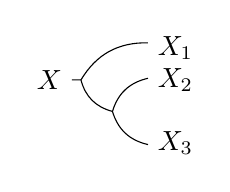
\begin{tikzpicture}[scale=0.8]
	\path (0,0) node (X) {$X$} 
	++ (0.5,0) coordinate (copy0)
	+ (1.5,0.5) node (X1) {$\RV{X}_1$}
	++ (0.5,-0.5) coordinate (copy1)
	+(1,0.5) node (X2) {$\RV{X}_2$}
	+(1,-0.5) node (X3) {$\RV{X}_3$};
	\draw (X) -- (copy0) to [bend left] (X1) (copy0) to [bend right] (copy1) to [bend left] (X2) (copy1) to [bend right] (X3);
	\end{tikzpicture}
	=
	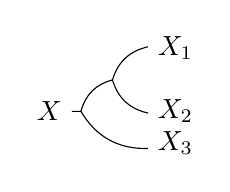
\begin{tikzpicture}[scale=0.8]
	\path (0,0) node (X) {$X$} 
	++ (0.5,0) coordinate (copy0)
	+ (1.5,-0.5) node (X1) {$\RV{X}_3$}
	++ (0.5,0.5) coordinate (copy1)
	+(1,0.5) node (X2) {$\RV{X}_1$}
	+(1,-0.5) node (X3) {$\RV{X}_2$};
	\draw (X) -- (copy0) to [bend right] (X1) (copy0) to [bend left] (copy1) to [bend left] (X2) (copy1) to [bend right] (X3);
	\end{tikzpicture}
	:=
	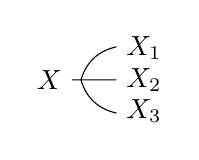
\begin{tikzpicture}[scale=0.8]
	\path (0,0) node (X) {$X$} 
	++ (0.5,0) coordinate (copy0)
	+ (1,0.5) node (X1) {$\RV{X}_1$}
	+(1,0) node (X2) {$\RV{X}_2$}
	+(1,-0.5) node (X3) {$\RV{X}_3$};
	\draw (X) -- (copy0) to [bend left] (X1) (copy0) to (X2) (copy0) to [bend right] (X3);
	\end{tikzpicture}\label{eq:ccom1}
\end{align}

\begin{align}
	\begin{tikzpicture}[scale=0.8]
	\path (0,0) node (X) {$X$}
	++(0.5,0) coordinate (copy0)
	+ (1,0.5) node (S) {}
	+(1,-0.5) node (X1) {$\RV{X}$};
	\draw (X) -- (copy0) to [bend right] (X1);
	\draw[-{Rays [n=8]}] (copy0) to [bend left] (S);
	\end{tikzpicture}
	= 
	\begin{tikzpicture}[scale=0.8]
	\path (0,0) node (X) {$X$}
	++(0.5,0) coordinate (copy0)
	+ (1,-0.5) node (S) {}
	+(1,0.5) node (X1) {$\RV{X}$};
	\draw (X) -- (copy0) to [bend left] (X1);
	\draw[-{Rays [n=8]}] (copy0) to [bend right] (S);
	\end{tikzpicture}
	=
	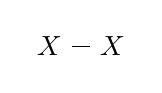
\begin{tikzpicture}[scale=0.8]
	\path (0,0) node (X) {$X$}
	++ (1,0) node (X1) {$\RV{X}$};
	\draw (X) -- (X1);
	\end{tikzpicture}\label{eq:ccom2}
\end{align}

\begin{align}
	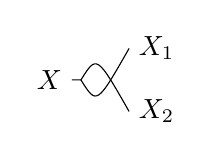
\begin{tikzpicture}[scale=0.8]
	\path (0,0) node (X) {$X$}
	++(0.5,0) coordinate (copy0)
	+ (1.2,0.5) node (X2) {$\RV{X}_1$}
	+(1.2,-0.5) node (X1) {$\RV{X}_2$};
	\draw (X) -- (copy0) .. controls (0.75,0.4) .. (X1.west);
	\draw (copy0) .. controls (0.75,-0.4) .. (X2.west);
	\end{tikzpicture}
=
	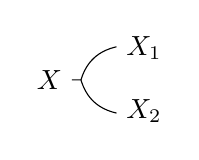
\begin{tikzpicture}[scale=0.8]
	\path (0,0) node (X) {$X$}
	++(0.5,0) coordinate (copy0)
	+ (1,0.5) node (X2) {$\RV{X}_1$}
	+(1,-0.5) node (X1) {$\RV{X}_2$};
	\draw (X) -- (copy0) to [bend right] (X1);
	\draw (copy0) to [bend left] (X2);
	\end{tikzpicture}\label{eq:ccom3}
\end{align}

The discard map $\stopper{0.2}$ can ``fall through'' any Markov kernel:

\begin{align}
\begin{tikzpicture}
\path (0,0) node (X) {$X$}
++(0.7,0) node[kernel] (A) {$\mathbf{A}$}
++(0.7,0) node (S) {};
\draw (X) -- (A);
\draw[-{Rays [n=8]}] (A) -- (S);
\end{tikzpicture}
= 
\begin{tikzpicture}
\path (0,0) node (X) {$X$}
++(0.7,0) node (S) {};
\draw[-{Rays [n=8]}] (X) -- (S);
\end{tikzpicture}\label{eq:termobj1}
\end{align}

Combining \ref{eq:ccom2} and \ref{eq:termobj1} we can derive the following: integrating $\mathbf{A}:X\to \Delta(\mathcal{Y})$ with respect to $\mu\in\Delta(\mathcal{X})$ and then discarding the output of $\mathbf{A}$ leaves us with $\mu$:

\begin{align}
\begin{tikzpicture}
\path (0,0) node[dist] (mu) {$\mu$}
++ (1,0) coordinate (copy0)
+ (1.4,0.5) node (X) {$\RV{X}$}
++ (0.7,-0.5) node[kernel] (A) {$\mathbf{A}$}
++(0.7,0) node (Y) {};
\draw (mu)--(copy0);
\draw (copy0) to [bend left] (X);
\draw[-{Rays [n=8]}] (copy0) to [bend right] (A) (A) -- (Y);
\end{tikzpicture}
= 
\begin{tikzpicture}
\path (0,0) node[dist] (mu) {$\mu$}
++ (1,0) coordinate (copy0)
+ (1.2,0.5) node (X) {$\RV{X}$}
++ (0.4,-0.3) coordinate (A)
++(0.1,0) node (Y) {};
\draw (mu)--(copy0);
\draw (copy0) to [bend left] (X);
\draw[-{Rays [n=8]}] (copy0) to [bend right] (A) (A) -- (Y);
\end{tikzpicture}
=
\begin{tikzpicture}
\path (0,0) node[dist] (mu) {$\mu$}
++ (1,0) node (X) {$\RV{X}$};
\draw (mu)--(X);
\end{tikzpicture}
\end{align}

In elementary notation, this is equivalent to the fact that, for all $B\in \mathcal{X}$, $\int_B \mathbf{A}(x;B)d\mu(x) = \mu(B)$.

The following additional properties hold for $\stopper{0.2}$ and $\splitter{0.1}$:

\begin{align}
\begin{tikzpicture}
\path (0,0) node (XY) {$E\times F$}
++ (1.5,0) node (Z) {};
\draw[-{Rays [n=8]}] (XY) -- (Z);
\end{tikzpicture} &=
\begin{tikzpicture}
\path (0,0) node (X) {$E$} 
++ (1,0) node (X1) {}
(0,-0.3) node (Y) {$F$}
++ (1,0) node (Y1) {};
\draw[-{Rays [n=8]}] (X) -- (X1);
\draw[-{Rays [n=8]}] (Y) -- (Y1);
\end{tikzpicture}
\end{align}
\begin{align}
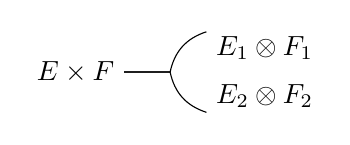
\begin{tikzpicture}
\path (0,0) node (XY) {$E\times F$}
++ (1.2,0) coordinate (copy0)
++(1.2,0.3) node (XY1) {$\RV{E}_1\otimes\RV{F}_1$}
++(0,-0.6) node (XY2) {$\RV{E}_2\otimes \RV{F}_2$};
\draw (XY) -- (copy0) to [bend left] (XY1);
\draw (XY) -- (copy0) to [bend right] (XY2);
\end{tikzpicture} &=
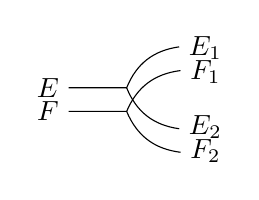
\begin{tikzpicture}
\path (0,0) node (XY) {$E$}
++ (1.,0) coordinate (copy0)
++(1.,0.5) node (XY1) {$\RV{E}_1$}
++(0,-1) node (XY2) {$\RV{E}_2$}
(0,-0.3) node (F) {$F$}
++(1.,0) coordinate (copy1)
++(1.,0.5) node (F1) {$\RV{F}_1$}
++(0,-1) node (F2) {$\RV{F}_2$};
\draw (XY) -- (copy0) to [bend left] (XY1);
\draw (copy0) to [bend right] (XY2);
\draw (F) -- (copy1) to [bend left] (F1);
\draw (copy1) to [bend right] (F2);
\end{tikzpicture}
\end{align}

A key fact that \emph{does not} hold in general is

\begin{align}
\begin{tikzpicture}
\path (0,0) node (E) {$E$}
++(0.5,0) coordinate (copy0)
++(0.7,0.3) node[kernel] (A1) {$\mathbf{A}$}
+(0,-0.6) node[kernel] (A2) {$\mathbf{A}$}
++(0.75,0) node (F1) {$\RV{F}_1$}
+(0,-0.6) node (F2) {$\RV{F}_2$};
\draw (E) -- (copy0) to [bend left] (A1) (A1) -- (F1);
\draw (copy0) to [bend right] (A2) (A2) -- (F2);
\end{tikzpicture} = \begin{tikzpicture}
\path (0,0) node (E) {$E$}
++ (0.7,0) node[kernel] (A) {$\mathbf{A}$}
++(0.7,0) coordinate (copy0)
++(0.5,0.3) node (F1) {$\RV{F}_1$}
+(0,-0.6) node (F2) {$\RV{F}_2$};
\draw (E) -- (A) -- (copy0) to [bend left] (F1);
\draw (copy0) to [bend right] (F2);
\end{tikzpicture} \label{eq:copy_commutes}
\end{align}

In fact, it holds only when $\mathbf{A}$ is a \emph{deterministic} kernel.

\begin{definition}[Deterministic Markov kernel]
A \emph{deterministic} Markov kernel $\mathbf{A}:E\to \Delta(\mathcal{F})$ is a kernel such that $\mathbf{A}_x(B)\in\{0,1\}$ for all $x\in E$, $B\in\mathcal{F}$.
\end{definition}

\begin{theorem}[Copy map commutes for deterministic kernels \citep{fong_causal_2013}]
Equation \ref{eq:copy_commutes} holds iff $\mathbf{A}$ is deterministic.
\end{theorem}

\paragraph{Disintegraion and Bayesian Inversion}\label{pgph:disint}

We use \emph{disintegration} to define a notion of conditional probability. It is not identical to the standard definition of conditional probability one can find in, for example, \citet{cinlar_probability_2011}, but each can be recovered from the other.

We'll proceed from an example to a general definition. 

\begin{example}[Disintegration with respect to ``convenient'' random variables]\label{ex:disintegration}
Given a probability measure $\mu\in \Delta(\mathcal{E}\otimes\mathcal{F}\otimes \mathcal{G})$:
\begin{align}
\begin{tikzpicture}
\path (0,0) node[dist] (m) {$\mu\;$}
++ (0.7,0.3) node (E) {$\RV{E}$}
++ (0,-0.3) node (F) {$\RV{F}$}
++(0,-0.3) node (G) {$\RV{G}$};
\draw ($(m.east) + (0,0.3)$) -- (E);
\draw ($(m.east) + (0,0)$) -- (F);
\draw ($(m.east) + (0,-0.3)$) -- (G);
\end{tikzpicture}
\end{align}

A Markov kernel $\mathbf{D}_{\RV{F}|\RV{E}}$ is a $\RV{F}|\RV{E}$ (``$\RV{F}$ on $\RV{E}$'')-disintegration of $\mu$ if

\begin{align}
\begin{tikzpicture}
\path (0,0) node[dist] (m) {$\mu\;$}
++ (0.7,0.3) node (E) {$\RV{E}$}
++ (0,-0.3) node (F) {$\RV{F}$}
++(0,-0.3) node (G) {};
\draw ($(m.east) + (0,0.3)$) -- (E);
\draw ($(m.east) + (0,0)$) -- (F);
\draw[-{Rays [n=8]}] ($(m.east) + (0,-0.3)$) -- (G);
\end{tikzpicture}=
\begin{tikzpicture}
\path (0,0) node[dist] (m) {$\mu\;$}
++ (0.7,0.3) coordinate (E) 
+ (0,-0.3) node (F) {}
+ (0,-0.6) node (G) {}
++ (0.5,0.15) coordinate (E1) 
+ (1.5,0) node (E2) {$\RV{E}$}
++ (0,-0.4) coordinate (F1)
++ (0.5,0) node[kernel] (D) {$\mathbf{D}_{\RV{F}|\RV{E}}$}
++ (1,0) node (F2) {$\RV{F}$};
\draw ($(m.east) + (0,0.3)$) -- (E);
\draw[-{Rays [n=8]}] ($(m.east) + (0,-0)$) -- (F);
\draw[-{Rays [n=8]}] ($(m.east) + (0,-0.3)$) -- (G);
\draw (E) to [out=45,in=180] (E1) -- (E2);
\draw (E) to [bend right] (F1) -- (D) -- (F2);
\end{tikzpicture}\label{eq:integrating_disintegration}
\end{align}

Equation \ref{eq:integrating_disintegration} echoes the familiar property of conditional probability $P(A\cap B) = P(A|B)P(B)$; in elementary notation it states that for and disintegration $\mathbf{D}_{\RV{F}|\RV{E}}$ and all $A\in\mathcal{E}$, $B\in \mathcal{F}$, $\mu(A\times B)= \int_A \mathbf{D}_{\RV{F}|\RV{E}}(x;B) d\mu_{\RV{E}} (x)$ where $\mu_{\RV{E}}:=\mu \mathbf{F}_{\RV{E}}$ is the marginal distribution of $\RV{E}$ under $\mu$.
\end{example}

Example \ref{ex:disintegration} defines disintegration given a probability measure $\mu$ and a pair of random variables $\RV{E}$ and $\RV{F}$ that are adapted to the product structure of the output space of $\mu$, a product structure that allows us to draw a diagram for $\mu$ featuring two wires as outputs. There are three extensions to this definition that are desirable:

\begin{enumerate}
\item We would like to replace individual wires $\RV{E}$ and $\RV{F}$ with arbitrary sets of wires
\item We would like to be able to disintegrate a probability mesure with respect to arbitrary random variables, not just sets that are adapted to the product structure of the output space
\item We would like to define disintegration for arbitrary Markov kernels rather than probability measures only
\end{enumerate}

As we show, we can associate any set of wires with a random variable, so the first item is solved by a solution to the second. 

\begin{definition}[Coupled tensor product $\utimes$]
Given two Markov kernels $\mathbf{M}$ and $\mathbf{N}$ or functions $f$ and $g$ with shared domain $E$, let $\mathbf{M}\utimes\mathbf{N}:=\splitter{0.1}(\mathbf{M}\otimes\mathbf{N})$ and $f\utimes g:=\splitter{0.1}(f\otimes g)$ where these expressions are interpreted using standard product notation. Graphically:

\begin{align}
\mathbf{M}\utimes\mathbf{N}&:=\begin{tikzpicture}
\path (0,0) node (E) {$E$}
++(0.5,0) coordinate (copy0)
+ (0.5,0.3) node[kernel] (M) {$\mathbf{M}$}
+(1.2,0.3) node (X) {$\RV{X}$}
+ (0.5,-0.3) node[kernel] (N) {$\mathbf{N}$}
+(1.2,-0.3) node (Y) {$\RV{Y}$};
\draw (E) -- (copy0) to [bend left] (M) (copy0) to [bend right] (N);
\draw (M) -- (X) (N) -- (Y);
\end{tikzpicture}\\
f\utimes g&:= \begin{tikzpicture}[scale=1.2]\path (0,0) node (E) {$E$}
++(0.5,0) coordinate (copy0)
+ (0.5,0.3) node[expectation] (M) {$f$}
+ (0.5,-0.3) node[expectation] (N) {$g$};
\draw (E) -- (copy0) to [bend left] (M) (copy0) to [bend right] (N);
\end{tikzpicture}
\end{align}

The operation denoted by $\utimes$ is associative (Lemma \ref{lem:utimes_assoc}), so we can without ambiguity write $f\utimes g\utimes ...\utimes h$ for finite groups of functions or Markov kernels sharing a domain. 
\end{definition}

\begin{lemma}[$\utimes$ is associative]\label{lem:utimes_assoc}
For Markov kernels $\mathbf{L}$, $\mathbf{M}$ and $\mathbf{N}$ sharing a domain $E$, $(\mathbf{L}\utimes\mathbf{M})\utimes\mathbf{N}=\mathbf{L}\utimes(\mathbf{M}\utimes\mathbf{N})$.
\end{lemma}

\begin{proof}
This follows from the commutativity of the swap map (Equation \ref{eq:ccom1}):

\begin{align}
	(\mathbf{L}\utimes\mathbf{M})\utimes\mathbf{N} &= \splitter{0.1}(\splitter{0.1}(\mathbf{L}\otimes\mathbf{M})\otimes\mathbf{N})\\
									   &= \begin{tikzpicture}[yscale=2,xscale=1.5]
									   \path (0,0) node (E) {$E$}
									   ++(0.5,0) coordinate (copy0)
									   +(0.5,0.25) coordinate (copy1)
									   +(0.5,-0.25) coordinate (Z0)
									   (copy1) ++(0.5,0.15) node[kernel] (X) {$\mathbf{L}$}
									   ++ (0,-0.3) node[kernel] (Y) {$\mathbf{M}$}
									   (Z0) ++ (0.5,0) node[kernel] (Z) {$\mathbf{N}$};
									   \draw (E) -- (copy0) to [bend left] (copy1) (copy0) to [bend right] (Z0) -- (Z);
									   \draw (copy1) to [bend left] (X) (copy1) to [bend right] (Y);
									   \draw (X) -- +(0.5,0) (Y) -- +(0.5,0) (Z) -- +(0.5,0);
									   \end{tikzpicture}\\
									   &= \begin{tikzpicture}[yscale=2,xscale=1.5]
   									   \path (0,0) node (E) {$E$}
									   ++(0.5,0) coordinate (copy0)
									   +(0.5,-0.25) coordinate (copy1)
									   +(0.5,0.25) coordinate (X0)
									   (X0) ++(0.5,0) node[kernel] (X) {$\mathbf{L}$}
									   ++ (0,-0.3) node[kernel] (Y) {$\mathbf{M}$}
									   (copy1) ++ (0.5,-0.25) node[kernel] (Z) {$\mathbf{N}$};
									   \draw (E) -- (copy0) to [bend right] (copy1) (copy0) to [bend left] (X0) -- (X);
									   \draw (copy1) to [bend right] (Z) (copy1) to [bend left] (Y);
   									   \draw (X) -- +(0.5,0) (Y) -- +(0.5,0) (Z) -- +(0.5,0);
									   \end{tikzpicture}\\
									   &= \mathbf{L}\utimes(\mathbf{M}\utimes\mathbf{N})
\end{align}
\end{proof}


\begin{definition}[Joint distribution]\label{def:joint_distribution}
Given $\mu\in \Delta(\mathcal{E})$ and $\RV{X}:E\to X$ and $\RV{Y}:E\to Y$, the \emph{joint distribution} of $\RV{X}$ and $\RV{Y}$ is the pushforward measure of $\mu$ by the random variable $\RV{X}\utimes\RV{Y}$ on $\mathcal{X}\otimes\mathcal{Y}$.

This is identical to the definition in, for example, \citet{cinlar_probability_2011} if we note that the random variable $(\RV{X},\RV{Y}):\omega\mapsto (\RV{X}(\omega),\RV{Y}(\omega))$ (\c{C}inlar's definition) is equivalent to $\RV{X}\utimes\RV{Y}$.
\end{definition}

\begin{lemma}[Joint distributions from coupled tensor products]\label{lem:rvg_jd}
Given a probability space $\langle E,\mathcal{E},\mu \rangle$ and a finite set of random variables $G = \{\RV{X}_i|i\in [n]\}$, the joint distribution of $G$ is given by $\mu (\utimes_{i\in [n]} \mathbf{F}_{\RV{X}_i})$.
\end{lemma}

\begin{proof}
This follows directly from Definition \ref{def:joint_distribution} and Lemma \ref{lem:pushf_funk}.
\end{proof}

\begin{lemma}\label{lem:thing_commutes}
For measurable functions $\RV{X}:E\to X$ and $\RV{Y}:E\to Y$, $\mathbf{F}_{\RV{X}\utimes\RV{Y}}=\mathbf{F}_{\RV{X}}\utimes\mathbf{F}_{\RV{Y}}$.
\end{lemma}

\begin{proof}
$\mathcal{X}\otimes\mathcal{Y}$ is by definition generated by the rectangles $A\times B$ for $A\in\mathcal{X}$, $B\in \mathcal{Y}$. To show equivalence of kernels $E\to \Delta(\mathcal{X}\otimes\mathcal{Y})$ it is sufficient to show agreement on all $s\in E$ and rectangles $A\times B$, $A\in \mathcal{X}$, $B\in \mathcal{Y}$.

For all $q\in X$, $r\in Y$, $A\in\mathcal{X}$ and $B\in \mathcal{Y}$, we have
\begin{align}
	\delta_{(q,r)}(A\times B) = \delta_q (A) \delta_r (B)
\end{align}

This can be verified by checking the four combinations of $q$ in or not in A and $r$ in or not in $B$.

For all $s\in E$, $A\in\mathcal{X},B\in\mathcal{Y}$,
\begin{align}
	\mathbf{F}_{\RV{X}\utimes\RV{Y}}(s;A\times B) &= \delta_{\RV{X}(s),\RV{Y}(s)}(A\times B)\\
												  &= \delta_{\RV{X}(s)}(A)\delta_{\RV{Y}(s)}(B)\\
												  &= (\mathbf{F}_{\RV{X}}\utimes \mathbf{F}_{\RV{Y}})(s;A\times B)
\end{align}
\end{proof}

\begin{definition}[Disintegration and Conditional Probability]
Given a probability measure $\mu\in \Delta(\mathcal{E})$:
\begin{align}
\begin{tikzpicture}
\path (0,0) node[dist] (m) {$\mu\;$}
++ (0.7,0) node (E) {$\RV{E}$};
\draw (m) -- (E);
\end{tikzpicture}
\end{align}

and two groups of random variables $G_X = \{\RV{X}_i|i\in[n]\}$ and $G_Y = \{\RV{Y}_i|i\in[m]\}$, define $\RV{X}=\utimes_{i\in[n]} \RV{X}_i$, $\RV{Y}:=\utimes_{i\in [m]} \RV{Y}_i$ and $\RV{W}=\RV{X}\utimes\RV{Y}$. Define the $\RV{X}|\RV{Y}$ disintegration of $\mu$ to be the $\RV{X}'|\RV{Y}'$ disintegration of $\mu \mathbf{F}_{\RV{W}}$, where $\RV{X}':\prod_{i\in [n]}X_i\times\prod_{j\in[m]}Y_j\to \prod_{i\in[n]}X_i$ and $\RV{Y}':\prod_{i\in [n]}X_i\times\prod_{j\in[m]}Y_j\to \prod_{i\in[n]}Y_i$ are the respective projection maps $\RV{X}':(x_0,...,x_[n],y_0,...,y_[m])\mapsto (x_0,...,x_m)$ and $\RV{Y}':(x_0,...,x_[n],y_0,...,y_[m])\mapsto (y_0,...,y_[m])$.

By construction, $\RV{X}'$ and $\RV{Y}'$ are such that $\RV{X}'\circ\RV{W}=\RV{X}$ and $\RV{Y}'\circ\RV{W} = \RV{Y}$.

By Lemma \ref{lem:thing_commutes}, $\mathbf{D}_{\RV{X}|\RV{Y}}$ is a $\RV{X}|\RV{Y}$ disintegration of $\mu$ if and only if
\begin{align}
\begin{tikzpicture}
\path (0,0) node[dist] (M) {$\mu$}
++ (0.5,0) coordinate (copy0)
++ (0.5,0.3) node[kernel] (FX) {$\mathbf{F}_{\RV{X}}$}
+  (0.7,0) node (XP) {$\RV{X}'$}
++ (0,-0.6) node[kernel] (FY) {$\mathbf{F}_{\RV{Y}}$}
+ (0.7,0) node (YP) {$\RV{Y}'$};
\draw (M) -- (copy0) to [bend left] (FX) (FX) -- (XP);
\draw (copy0) to [bend right] (FY) (FY) -- (YP);
\end{tikzpicture} &= 
\begin{tikzpicture}
\path (0,0) node[dist] (M) {$\mu$}
++ (0.7,0) node[kernel] (FY) {$\mathbf{F}_{\RV{Y}}$}
++(0.7,0) coordinate (copy0)
++ (0.7,0.3) node[kernel] (FX) {$\mathbf{D}_{\RV{X}|\RV{Y}}$}
+(0.8,0) node (XP) {$\RV{X}'$}
++(0,-0.6) coordinate (YY)
+ (0.8,0) node (YP) {$\RV{Y}'$};
\draw (M) -- (FY) -- (copy0) to [bend left] (FX) (FX) -- (XP);
\draw (copy0) to [bend right] (YY) (YY) -- (YP);
\end{tikzpicture}\label{eq:proper_disintegration}
\end{align}

Equation \ref{eq:proper_disintegration} generalises \ref{eq:integrating_disintegration} beyond disintegrations by ``convenience'' wire labels to disintegrations by arbitrary sets of random variables. Note that where we \emph{can} construct a diagram for $\mu$ with convenient labels for $\RV{X}$ and $\RV{Y}$, due to the identification between random variables and wires, $\ref{eq:proper_disintegration}$ reduces to $\ref{eq:integrating_disintegration}$, and we will use the simpler definition where possible as it yields less cluttered diagrams.


From the fact that $\mathbf{F}_{\RV{Y}}$ is a deterministic kernel, we also have:

\begin{align}
\begin{tikzpicture}
\path (0,0) node[dist] (M) {$\mu$}
++ (0.7,0) node[kernel] (FY) {$\mathbf{F}_{\RV{Y}}$}
++(0.7,0) coordinate (copy0)
++ (0.7,0.3) node[kernel] (FX) {$\mathbf{D}_{\RV{X}|\RV{Y}}$}
+(0.8,0) node (XP) {$\RV{X}'$}
++(0,-0.6) coordinate (YY)
+ (0.8,0) node (YP) {$\RV{Y}'$};
\draw (M) -- (FY) -- (copy0) to [bend left] (FX) (FX) -- (XP);
\draw (copy0) to [bend right] (YY) (YY) -- (YP);
\end{tikzpicture}\\
&= \begin{tikzpicture}
\path (0,0) node[dist] (M) {$\mu$}
++(0.7,0) coordinate (copy0)
++ (0.7,0.3) node[kernel] (FY1) {$\mathbf{F}_{\RV{Y}}$}
+ (0,-0.6) node[kernel] (FY) {$\mathbf{F}_{\RV{Y}}$}
++ (0.8,0) node[kernel] (FX) {$\mathbf{D}_{\RV{X}|\RV{Y}}$}
+(0.8,0) node (XP) {$\RV{X}'$}
+ (0.8,-0.6) node (YP) {$\RV{Y}'$};
\draw (M) -- (copy0) to [bend left] (FY1) (FY1) -- (FX) -- (XP);
\draw (copy0) to [bend right] (FY) (FY) -- (YP);
\end{tikzpicture}
\end{align}

We note, without proof, that: $\mathbf{F}_{\RV{Y}} \mathbf{D}_{\RV{X}|\RV{Y}}$ is an ordinary conditional probability $\mu(\RV{X}|\otimes_{i\in[m]}\mathcal{Y}_i)$, and where such an ordinary conditional probability exists we can find a disintegration $\mathbf{D}_{\RV{X}|\RV{Y}}$ \citep{cinlar_probability_2011}.

In addition, it is well known that disintegrations of $\mu$ are non-unique, and different disintegrations are equal only up to sets of $\mu$-measure 0. This ambiguity turns out to be more problematic in our causal work as sets of $\mu$-measure 0 may meaningfully impact the consequences of decisions in fairly ordinary circumstances.
\end{definition}

We are also interested in an analogue of disintegration that applies to an arbitrary Markov kernel $\mathbf{M}:E\to \Delta(\mathcal{F})$ rather than only to probability measures. A generalised notion of disintegraion will allow for a formal definition of \citet{dawid_beware_2010}'s definition of ``extended conditional independence''. 

There are a number of choices we could make here, and we have made a particular choice that leads to generalised disintegrations usually failing to exist. This choices allows for a much cleaner treatment of conditional independence, as we will explain below.

\begin{definition}[Generalised Disintegration]
Given a Markov kernel $\mathbf{M}:E\to \Delta(\mathcal{F})$ and random variables $\RV{X}:F\to X$, $\RV{Y}:F\to Y$, a $\RV{X}|\RV{Y}$ disintegration of $\mathbf{M}$ is any kernel $\mathbf{D}_{\RV{X}|\RV{Y}}$ such that
\begin{align}
\begin{tikzpicture}
\path (0,0) node (E) {$E$}
++(0.7,0) node[kernel] (M) {$\mathbf{M}$}
++ (0.5,0) coordinate (copy0)
++ (0.5,0.3) node[kernel] (FX) {$\mathbf{F}_{\RV{X}}$}
+  (0.7,0) node (XP) {$\RV{X}'$}
++ (0,-0.6) node[kernel] (FY) {$\mathbf{F}_{\RV{Y}}$}
+ (0.7,0) node (YP) {$\RV{Y}'$};
\draw (E)-- (M) -- (copy0) to [bend left] (FX) (FX) -- (XP);
\draw (copy0) to [bend right] (FY) (FY) -- (YP);
\end{tikzpicture} &= 
\begin{tikzpicture}
\path (0,0) node (E) {$E$}
++(0.7,0) node[kernel] (M) {$\mathbf{M}$}
++ (0.7,0) node[kernel] (FY) {$\mathbf{F}_{\RV{Y}}$}
++(0.7,0) coordinate (copy0)
++ (0.7,0.3) node[kernel] (FX) {$\mathbf{D}_{\RV{X}|\RV{Y}}$}
+(0.8,0) node (XP) {$\RV{X}'$}
++(0,-0.6) coordinate (YY)
+ (0.8,0) node (YP) {$\RV{Y}'$};
\draw (E)--(M) -- (FY) -- (copy0) to [bend left] (FX) (FX) -- (XP);
\draw (copy0) to [bend right] (YY) (YY) -- (YP);
\end{tikzpicture}
\end{align}

Similarly to the standard definition, this reduces in the case that $\mathbf{M}$ can be drawn with $\RV{X}$ and $\RV{Y}$ labelling output wires.
\end{definition}


\begin{example}[Generalised disintegrations usually do not exist]
Let $\mathbf{M}:\{0,1\}\to \Delta(\{0,1\}^2)$ be defined by $\mathbf{M}:q\mapsto \delta_q\otimes\delta_1$ and let $\RV{X}_0,\RV{X}_1:\{0,1\}^2\to\{0,1\}$ be defined by $\RV{X}_0:(r,s)\mapsto r$ and $\RV{X}_1:(r,s)\mapsto s$. Note that we can write:
\begin{align}
\begin{tikzpicture}
\path (0,0) node (E) {$\{0,1\}$}
++(1,0) node[kernel] (M) {$\mathbf{M}$}
+(0.8,0.15) node (X0) {$\RV{X}_0$}
+(0.8,-0.15) node (X1) {$\RV{X}_1$};
\draw (E) -- (M) ($(M.east)+(0,0.15)$) -- (X0);
\draw ($(M.east)+(0,-0.15)$) -- (X1);
\end{tikzpicture}
\end{align}

Suppose we have some $\mathbf{D}_{\RV{X}_0|\RV{X}_1}$. Then we must have 

\begin{align}
\delta_0 &= \begin{tikzpicture}
\path (0,0) node[dist] (E) {$\delta_0$}
++(1,0) node[kernel] (M) {$\mathbf{M}$}
+(0.8,0.15) node (X0) {}
++(1,-0.22) node[kernel] (D) {$\mathbf{D}_{\RV{X}_0|\RV{X}_1}$}
++(1,0) node (X1) {$\RV{X}_0$};
\draw[-{Rays [n=8]}] (E) -- (M) ($(M.east)+(0,0.15)$) -- (X0);
\draw ($(M.east)+(0,-0.15)$) -- (D) -- (X1);
\end{tikzpicture}\\
\delta_1 &= \begin{tikzpicture}
\path (0,0) node[dist] (E) {$\delta_1$}
++(1,0) node[kernel] (M) {$\mathbf{M}$}
+(0.8,0.15) node (X0) {}
++(1,-0.22) node[kernel] (D) {$\mathbf{D}_{\RV{X}_0|\RV{X}_1}$}
++(1,0) node (X1) {$\RV{X}_0$};
\draw[-{Rays [n=8]}] (E) -- (M) ($(M.east)+(0,0.15)$) -- (X0);
\draw ($(M.east)+(0,-0.15)$) -- (D) -- (X1);
\end{tikzpicture}
\end{align}

but by assumption

\begin{align}
\delta_1 = \begin{tikzpicture}
\path (0,0) node[dist] (E) {$\delta_0$}
++(1,0) node[kernel] (M) {$\mathbf{M}$}
+(0.8,0.15) node (X0) {}
++(1,-0.15) node (X1) {$\RV{X}_1$};
\draw[-{Rays [n=8]}] (E) -- (M) ($(M.east)+(0,0.15)$) -- (X0);
\draw ($(M.east)+(0,-0.15)$) -- (X1);
\end{tikzpicture} = \begin{tikzpicture}
\path (0,0) node[dist] (E) {$\delta_1$}
++(1,0) node[kernel] (M) {$\mathbf{M}$}
+(0.8,0.15) node (X0) {}
++(1,-0.15) node (X1) {$\RV{X}_1$};
\draw[-{Rays [n=8]}] (E) -- (M) ($(M.east)+(0,0.15)$) -- (X0);
\draw ($(M.east)+(0,-0.15)$) -- (X1);
\end{tikzpicture}
\end{align}

Thus no such $\mathbf{D}_{\RV{X}_0|\RV{X}_1}$ can exist.
 
\end{example}

% \begin{align}
% \begin{tikzpicture}
% \path (0,0) node[dist] (mu) {$\mu$}
% ++ (1,0) coordinate (copy0)
% + (1.2,0.5) node (X) {$\RV{X}$}
% ++ (0.5,-0.5) node[kernel] (A) {$\mathbf{A}$}
% ++(0.7,0) node (Y) {$\RV{Y}$};
% \draw (mu)--(copy0);
% \draw (copy0) to [bend left] (X);
% \draw (copy0) to [bend right] (A) (A) -- (Y);
% \end{tikzpicture}\qquad
% \begin{tikzpicture}
% \path (0,0) node[dist] (mu) {$\mu$}
% ++ (1,0) coordinate (copy0)
% + (1.2,0.5) node (X) {$\RV{X}$}
% ++ (0.5,-0.5) node[kernel] (A) {$\mathbf{A}$}
% ++(0.7,0) node (Y) {};
% \draw (mu)--(copy0);
% \draw (copy0) to [bend left] (X);
% \draw[-{Rays [n=8]}] (copy0) to [bend right] (A) (A) -- (Y);
% \end{tikzpicture}=
% \begin{tikzpicture}
% \path (0,0) node[dist] (MU) {$\mu$}
% + (0.5,0) node (X) {$\RV{X}$};
% \draw (MU) -- (X);
% \end{tikzpicture}\label{eq:jdist}
% \end{align}


